% Chapter Template
\chapter{Audio Processing} % Main chapter title

\label{Chapter5} % Change X to a consecutive number; for referencing this chapter elsewhere, use \ref{ChapterX}
Before we feed the audio clip to our machine learning model, it is crucial to pre-process the signal as to achieve higher accuracy
and avoid further deterioration.
The choice and implementation of noise filter will then be explained in \textbf{LINK TO SECTION 1}. We then feed the filtered output 
to a pitch detection algorithm (PDA) \textbf{lINK TO SECTION 2} and then a key detection algorithm (KDA) \textbf{LINK TO SECTION 3}
Figure \textbf{UPDATE!} shows the flowchart of the audio processing part of our project.

% \begin{tikzpicture}[>=latex', overlay]
% 	\tikzset{
% 		block/.style= {draw, rectangle, fill=white, align=center,minimum width=2cm,minimum height=1cm},
%         fbox/.style = {rectangle, draw, densely dashed, inner sep=4mm},
% 		input/.style={ % requires library shapes.geometric
%         draw,
%         trapezium,
%         trapezium left angle=60,
%         trapezium right angle=120,
%         minimum width=2cm,
%         align=center,
%         minimum height=1cm},
%     }

% 	\node (n1) [block]  {User sings into our app\\ 
%                  (Obtain input audio signal)}; 
% 	%\node (n2) [block, right=1cm of n1] 
%     %            {Trim silence at the start/\\end of audio clip};
% 	% \node (n3) [block, right=1cm of n1] 
%     %             {Implement noise filter};
% 	\node (n4) [block, right=1cm of n1]
%                 {Spectral reduction};
% 	\node (n5) [block, right=0.5cm of n4]
% 				{Low-pass filter};
% 	\begin{scope}[blend mode=overlay,overlay]
% 		\node (n3) [fbox, fit=(n4) (n5), fill=beige]  
% 				{Implement noise filter};
% 	\end{scope}
% 	\node (n6) [block, below=1.8cm of n1] 
%                 {Implement PDA};
% 	\node (n7) [block, right=1cm of n6] 
%                 {Implement KDA};
% 	\node (n8) [block, draw=red, right=1cm of n7]
%                 {Pass the output to Ed's ML model\\
% 				(Notes and keys)};
% 	\node [coordinate, below right =1cm and 4cm of n5] (right) {};  %% Coordinate on right and middle
% 	\node [coordinate, above left =1cm and 1cm of n6] (left) {};  %% Coordinate on left and middle
% 	\path[draw,->]   (n1) edge (n3)
%         		%(n2) edge (n3)
%         		(n3) edge (n4)
% 				(n4) edge (n5)
%         		(n5) -| (right) -- (left) |-  (n6)
%         		(n6) edge (n7)
% 				(n7) edge (n8);
% \end{tikzpicture}

%----------------------------------------------------------------------------------------
%	SECTION 0
%----------------------------------------------------------------------------------------
\section{Assumptions}
Before we delineate the approach to audio processing, there are some assumptions that our model
is built on:
\begin{itemize}
	\item \textbf{Assumption 1:} Users' audio input device does not contain active noise cancelling functions.
\end{itemize}

These assumptions will be referred to later on in the section.
%----------------------------------------------------------------------------------------
%	SECTION 1
%----------------------------------------------------------------------------------------
\section{Noise Filter}
Noise filtering is essential as it reducess or eliminates the noise present in the input signal.
A conventional method to quantify noise is to use signal-to-noise ratio (SNR), which is often 
represented in decibels.
\[SNR=10*log_10((P_{signal})/(P_{noise}))\]
As its name suggests, SNR is the power ratio between desired signal and undesired noise. Effectively,
we would like to use noise filters to achieve a higher SNR.\\ 
There is a few sources of noise when an user record himself with a microphone.
Firstly, there exists self-noise, which is the instrument noise produced by the microphone itself.
Noise may be induced or created when the signal passes through electronic componenets like transistors 
and printed circuit boards.\cite{selfnoise} 
The second source, ambient noise, contributes to a large portion of noise present in a recording.
Room reflections, extraneous noise, electromagnetic interference and mechanical noise are some causes 
to the existence of ambient noise. 

%-----------------------------------
%	SUBSECTION 1
%-----------------------------------
\subsection{Possible Models}
Most of the noise filters work in the frequency and spectral domain, here we are going to inspect and
compare 3 noise reduction mechanisms.

\begin{enumerate}
	\item Low-pass filter (LPF)\\
	LPF passes signals with \(f<f_{c}\), where \(f_{c}\) is the cut-off frequency, and attenuates
	signals with \(f>fc\). 
	\[H(f) = rect(f/(2*B))\]
	\[h(t))= \mathfrak{F}^-1{H(f)} = \int_{-B}^{B} e^(2(\pi)ift)\,df = 2Bsinc(2Bt)\]
	In order to implement an LPF, we have to transform signal from time domain to 
	frequency domain using fourier transform. An ideal LPF would completely remove frequencies that are
	higher than \(f_{c}\) and is a non-ca)sual linear time-invariant system. The impulse
	response of an LPF is a sinc function that extends to [$\infty$,-$\infty$]. This is why it is impossible to 
	realize an ideal LPF since that will take infinite time and memory.\\
	LPF avoids aliasing since it removes the high-frequency content but not the desired signal

	\item Wavelet transform\\
	Wavelet transform creates a representation of the signal in both time and frequency domain so localized 
	information of the signal can be efficiently accessed. It is often compared with fourier transform (FT), which
	has the below limitations: 
	\begin{enumerate}
		\item For windowed FT, if the feature is larger or shorter than the window, it cannot be captured completely.
		\item Time resolution for high frequencies is the same for low frequencies. As frequency increases, rate of 
		change of the signal increases, and high frequency signals contain more information in a window than that of 
		low frequency, thus we need a higher time resolution for that.
	\end{enumerate}
	Wavelet transform analyzes a signal by its different frequency components at multiple resolution so features that are 
	undiscovered at one resolution may be obvious at another. There are mainly 2 types of wavelet transforms, namely 
	continuous wavelet transform (CWT) and discrete wavelet transform (DWT) and here are the mathematical representations
	for the two transforms:
	CWT finds how alike a wavelet is in a signal, given the above 2 properties that the wavelet has. \cite{wavelet}
	This can be found by convolving the mother wavelet with our signal.

	\begin{equation*} 
		\text{CWT}(\mathrm{a},\mathrm{b}; \mathrm{x}(\mathrm{t}),\psi(\mathrm{t}))=\int_{-\infty}^{\infty}[\mathrm{x}(\mathrm{t})\frac{1}{\mathrm{a}}-\psi^{*}(\frac{\mathrm{t}-\mathrm{b}}{\mathrm{a}})]\text{dt}
	\end{equation*}\cite{wavelet_denoise}

	where $x(t)$ is the original signal, $\psi(t)$ is the mother wavelet, $a$ is a dilation parameter and $b$ is a translation parameter.
	Dilation factor represents how dispersed the wavelet is (similar to scaling) while translation factor tells us where the wavelet is
	positioned in time (similar to shifting). 
	
	\begin{figure}
		\centering
		\begin{subfigure}{.3\textwidth}
		  \centering
		  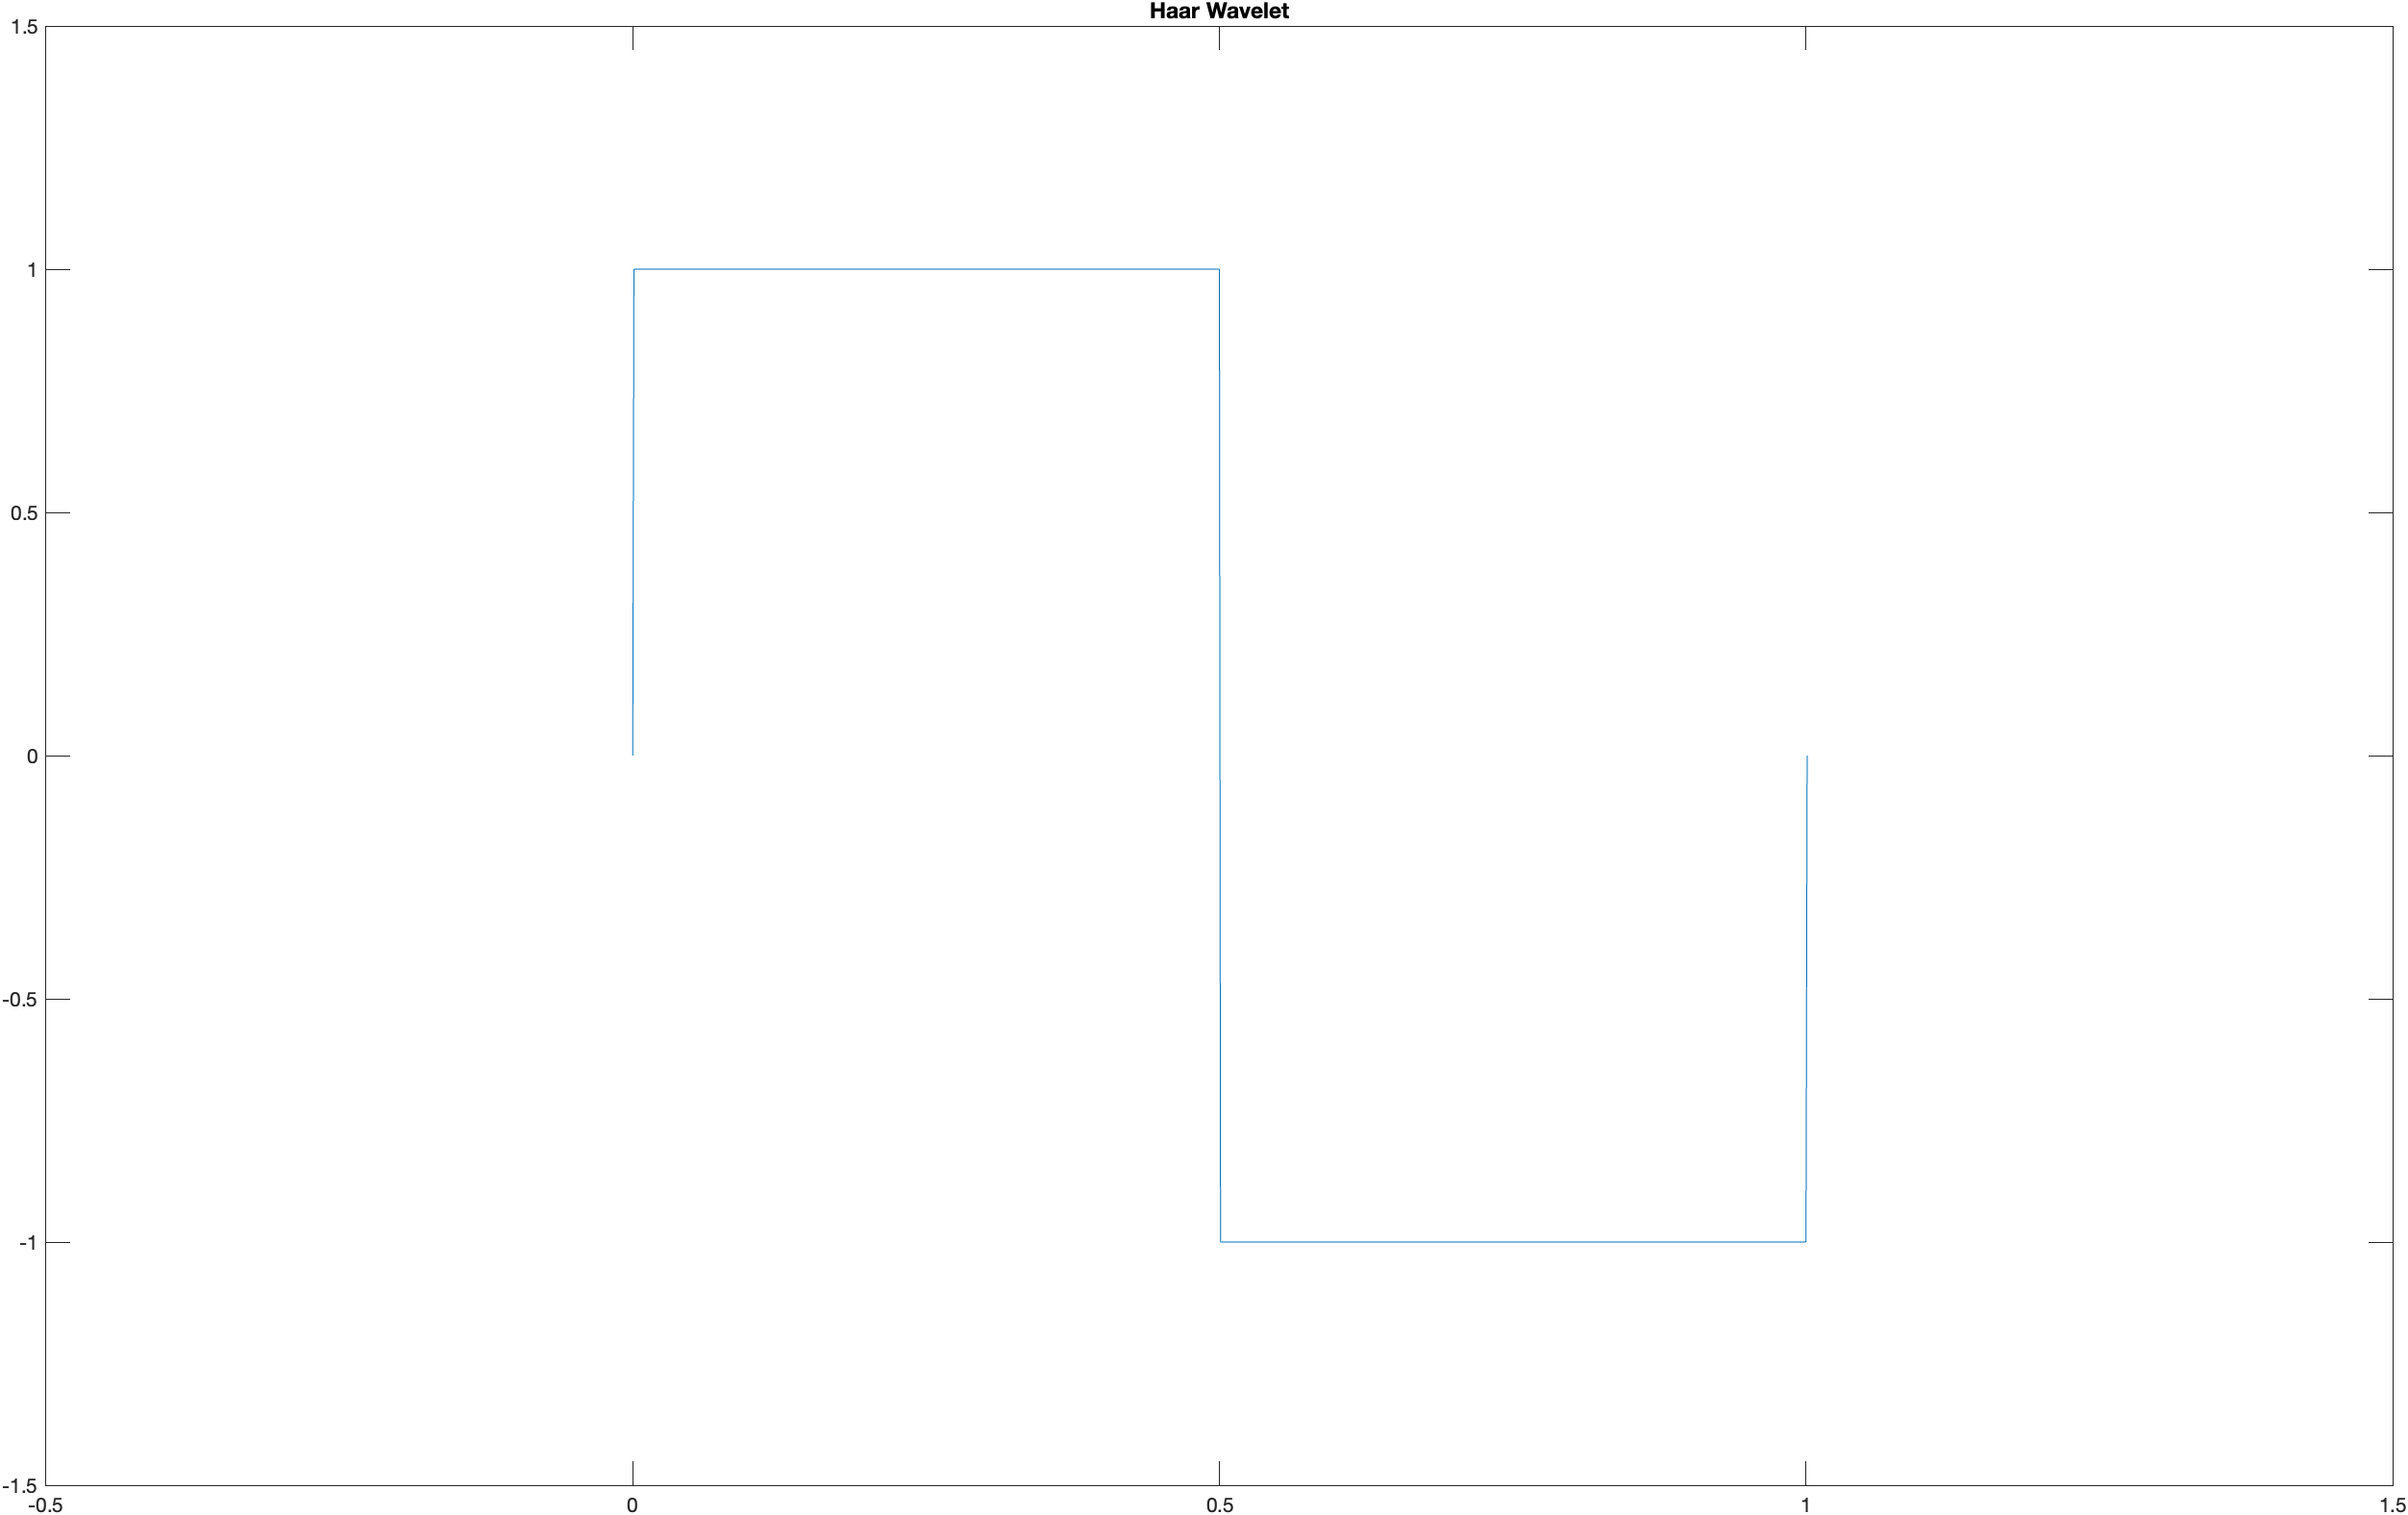
\includegraphics[width=1.1\linewidth]{haar.png}
		  \caption{Haar wavelet}
		  \label{Haar}
		\end{subfigure}%
		\begin{subfigure}{.3\textwidth}
			\centering
			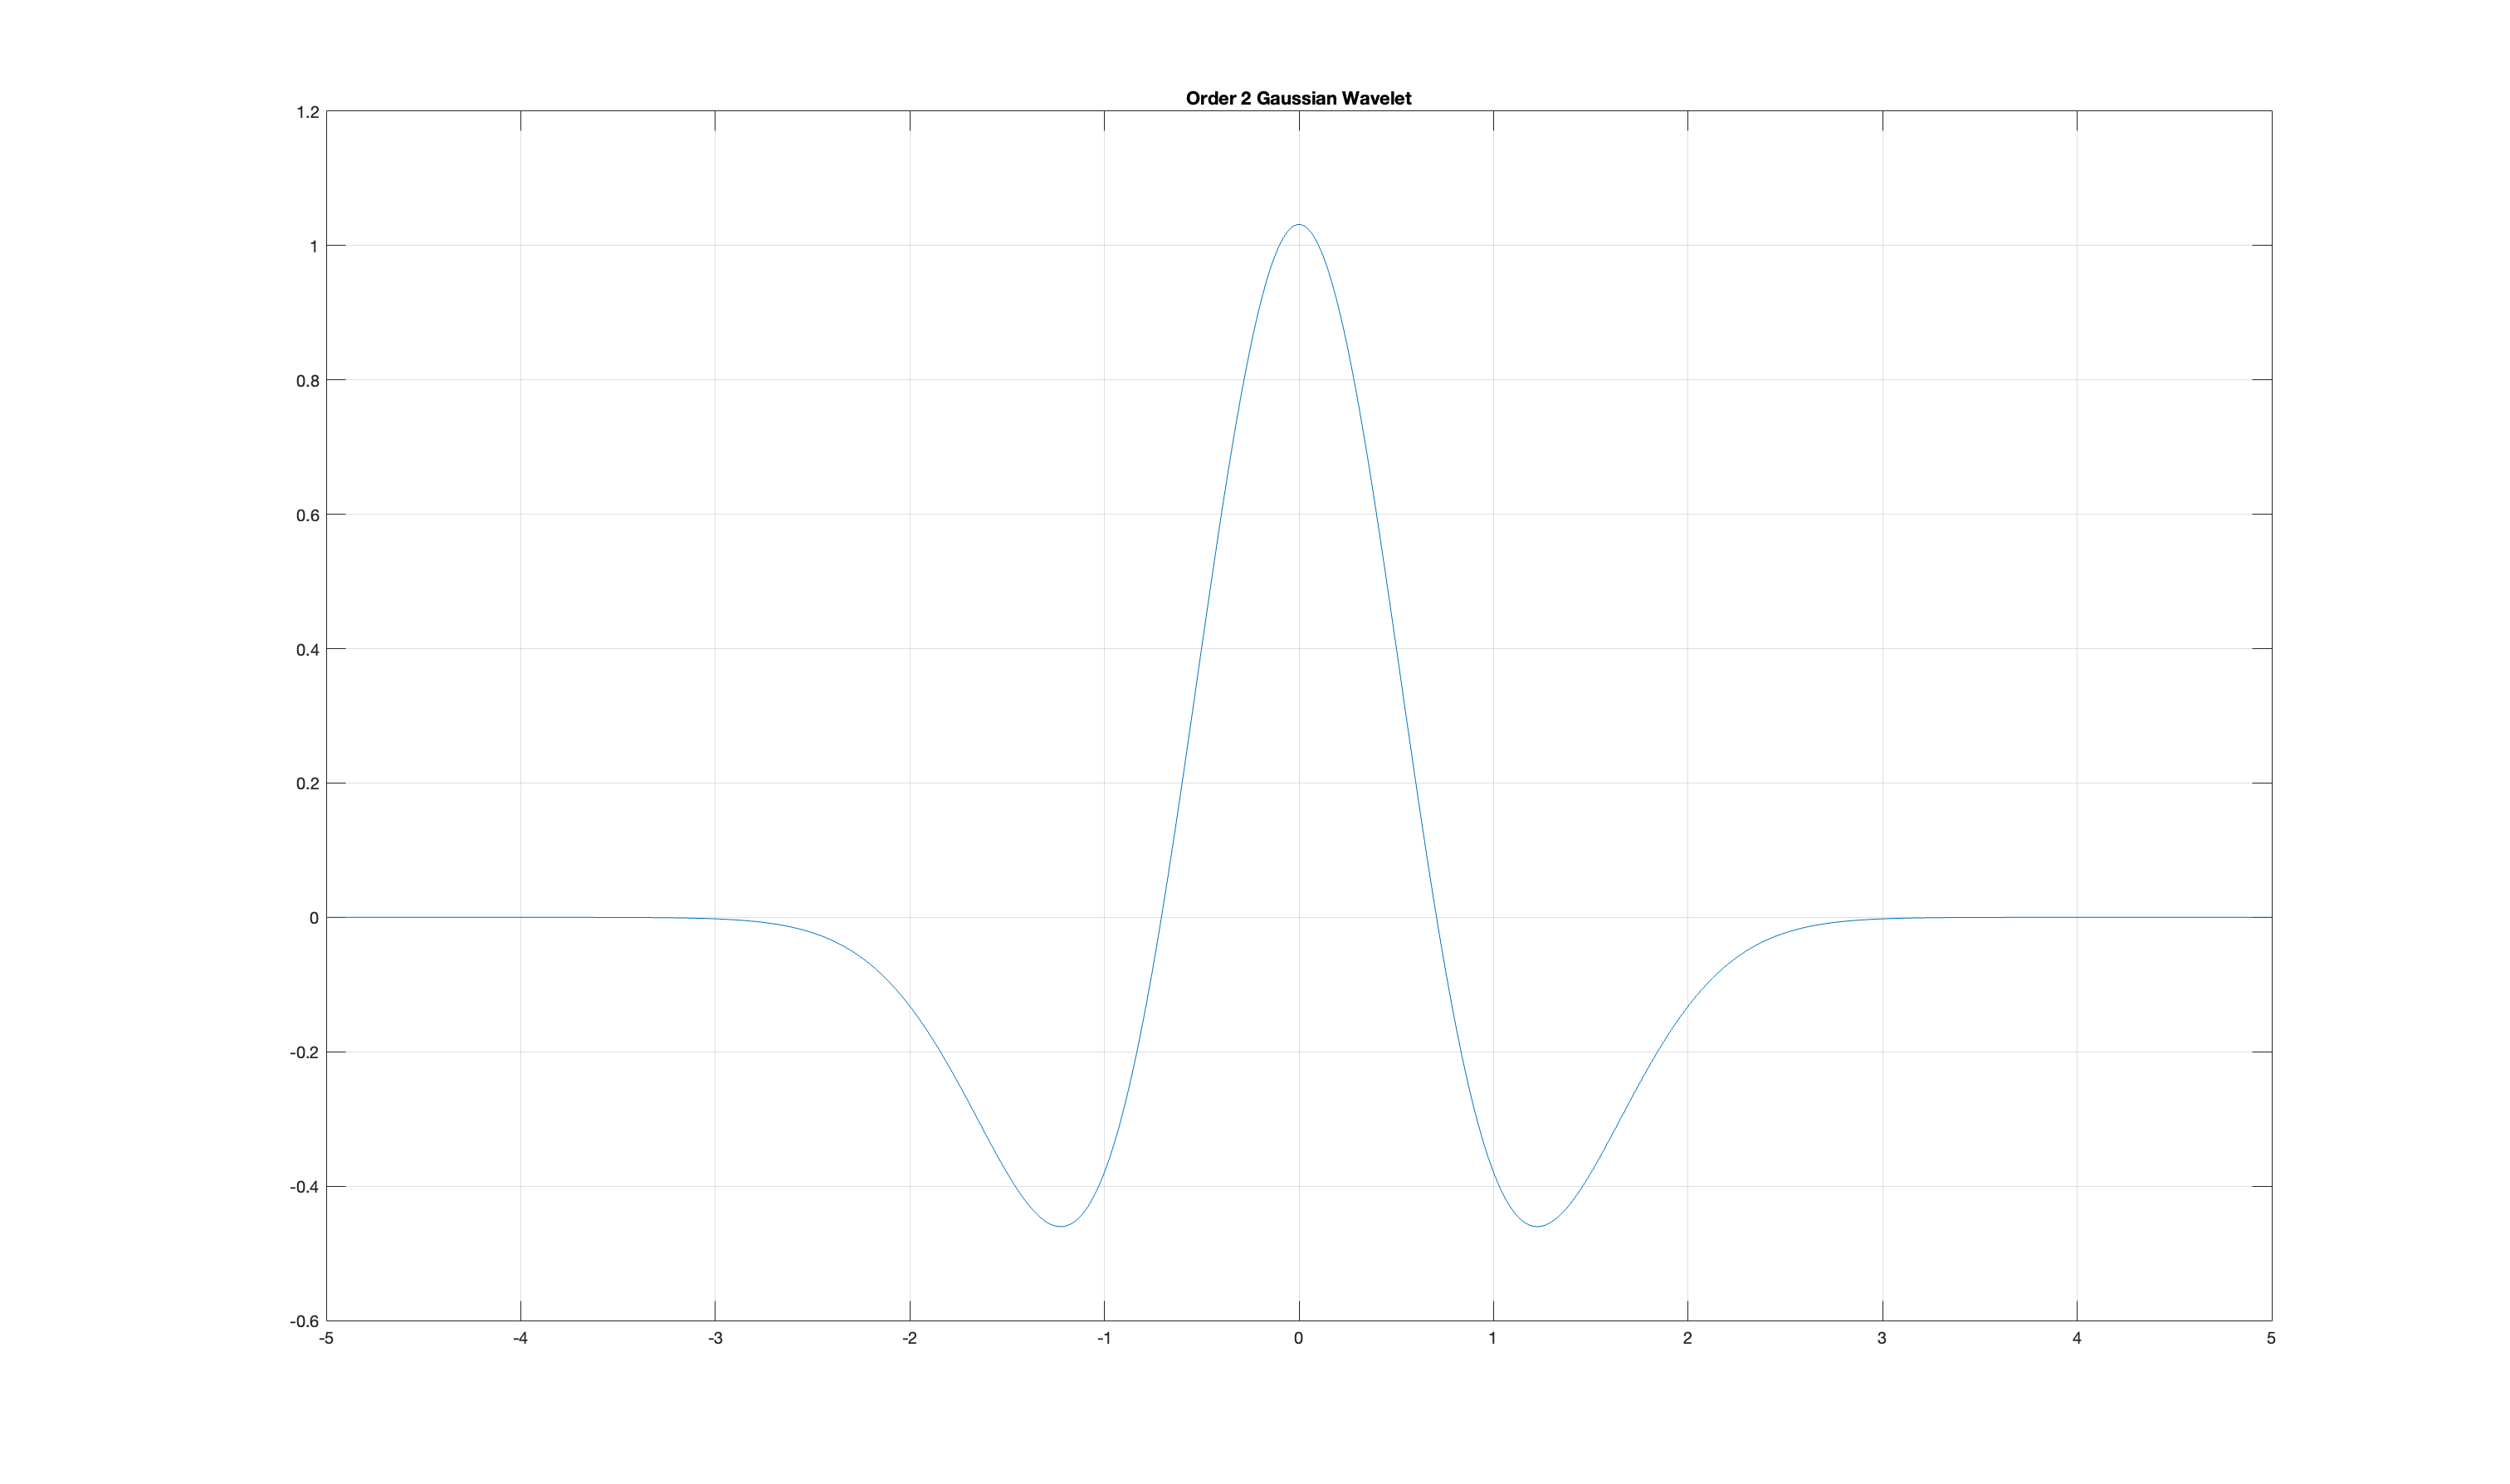
\includegraphics[width=1.1\linewidth]{order2gaussian.png}
			\caption{Gaussian wavelet of order 1}
			\label{order1}
		  \end{subfigure}%
		\begin{subfigure}{.3\textwidth}
		  \centering
		  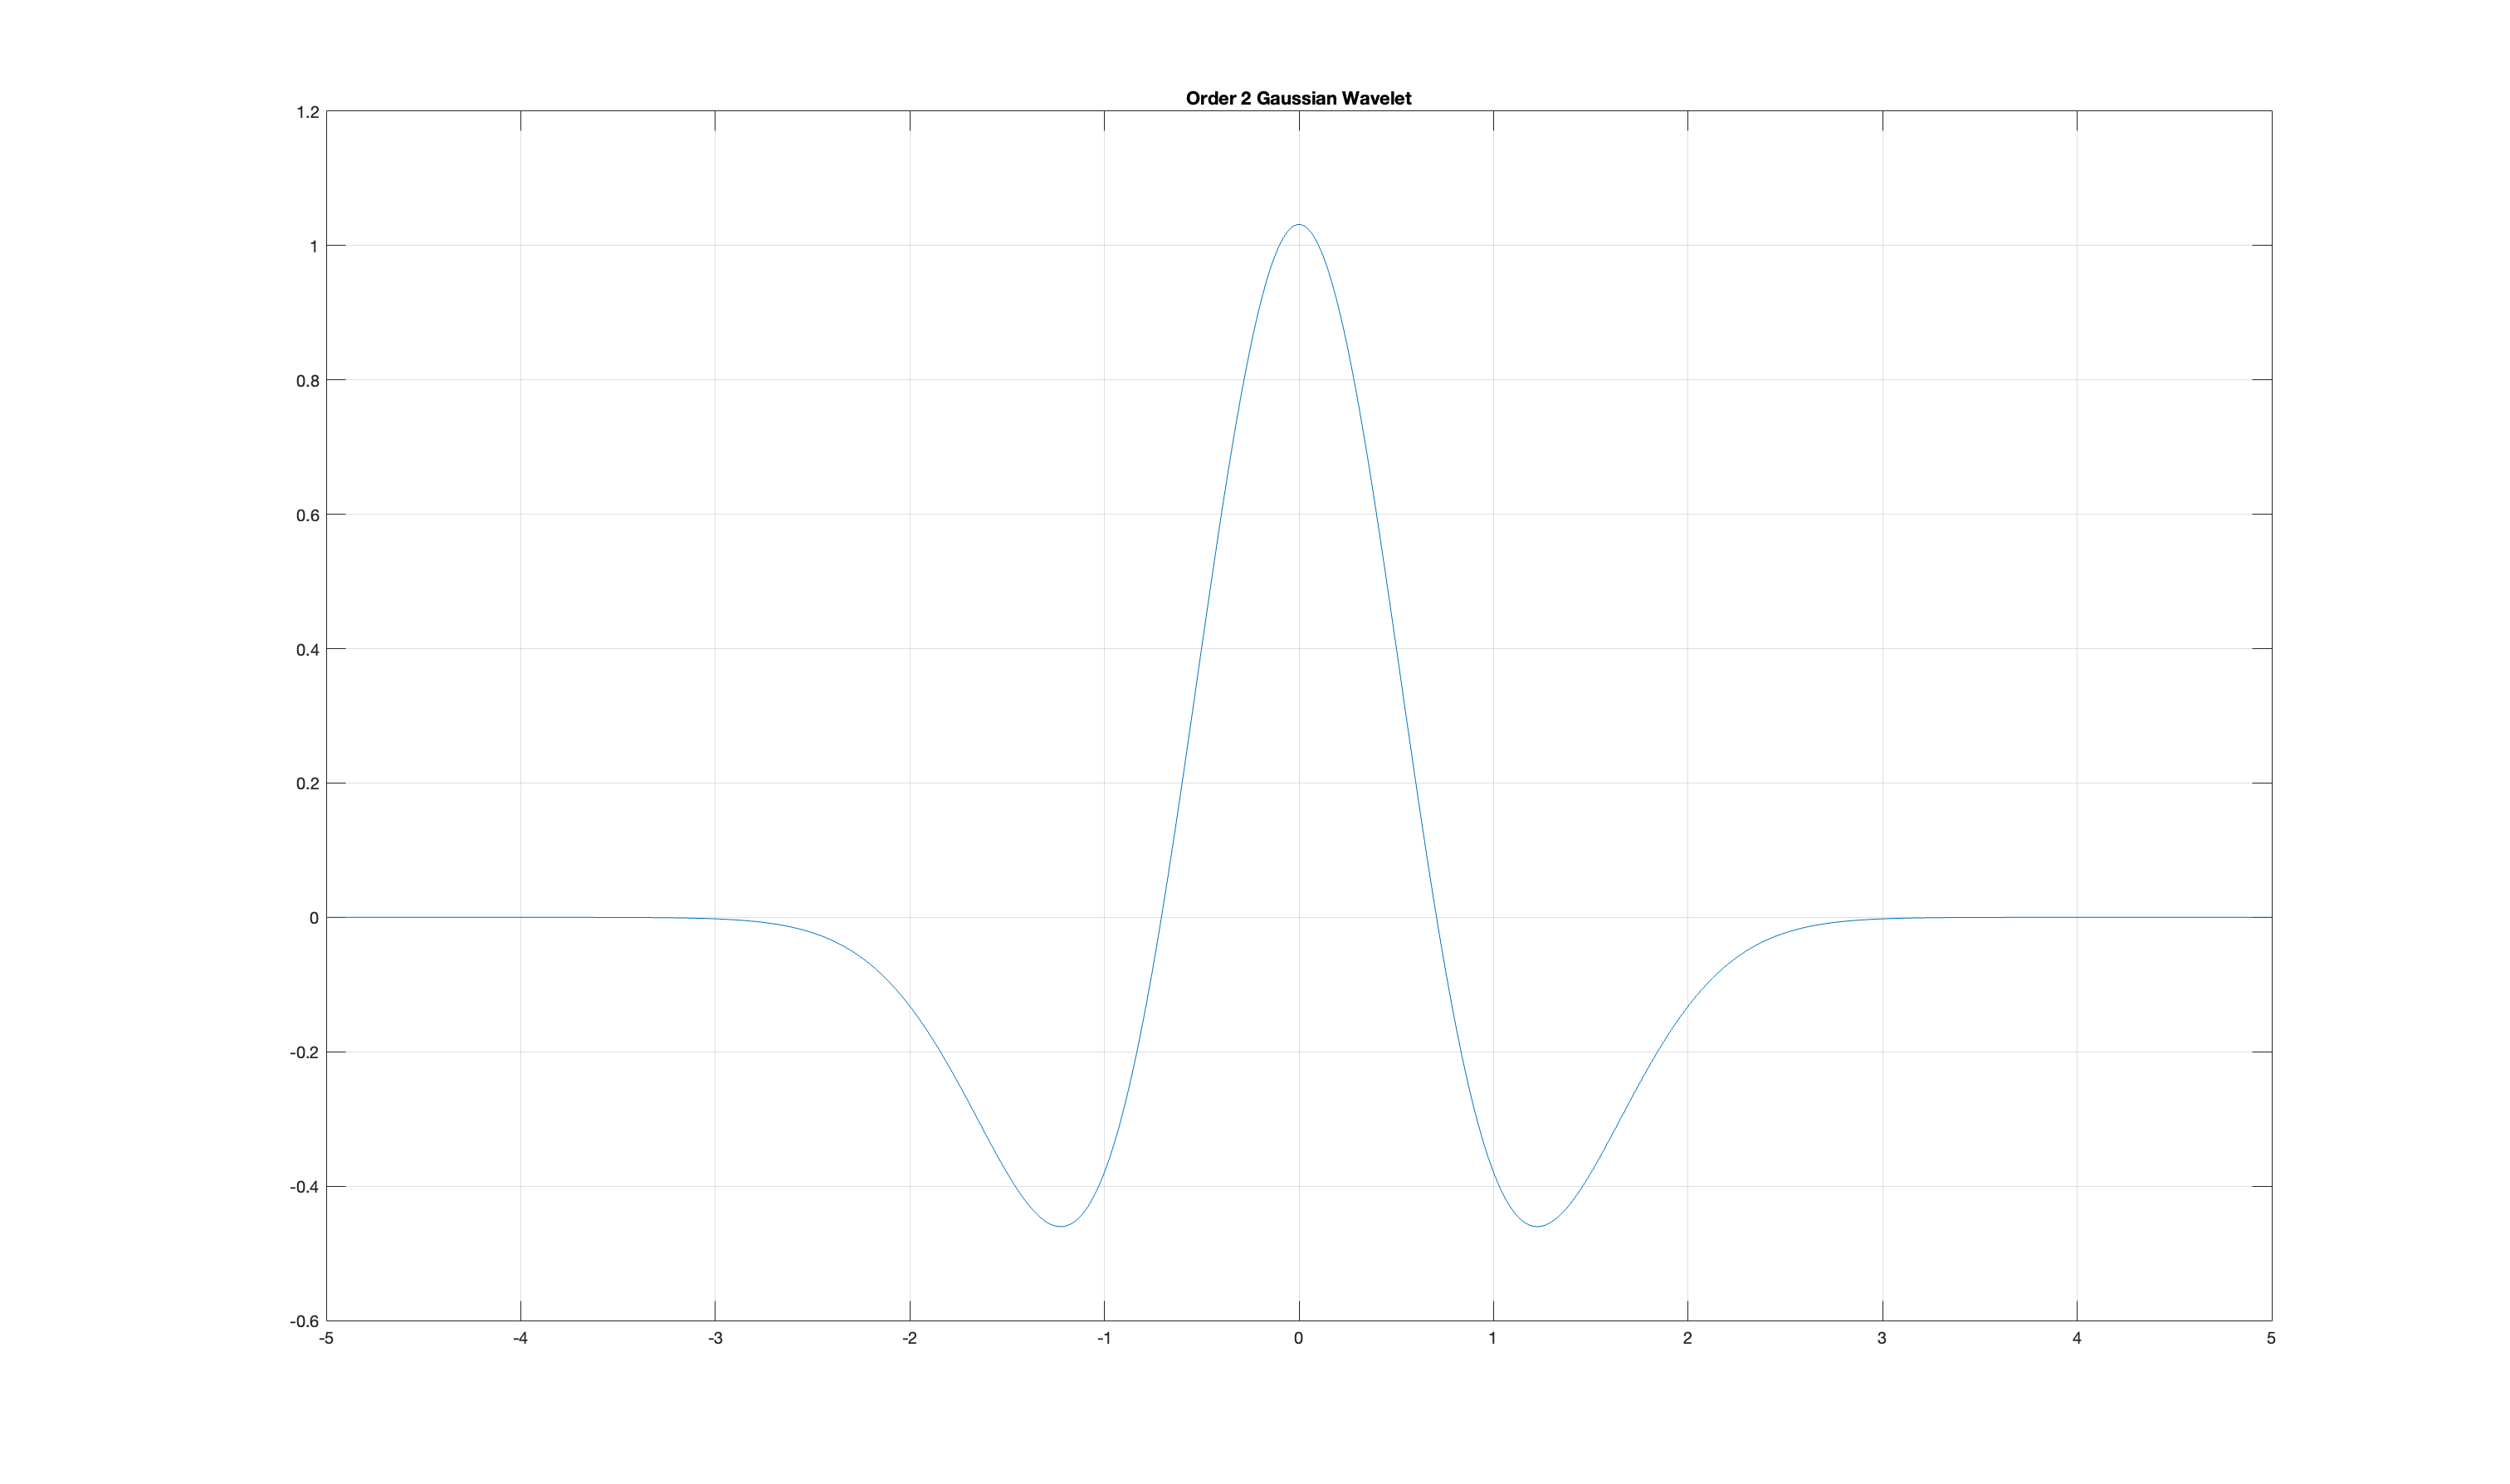
\includegraphics[width=1.1\linewidth]{order2gaussian.png}
		  \caption{Ricker wavelet - Gaussian wavelet of order 2}
		  \label{Ricker}
		\end{subfigure}%
		\caption{Examples of wavelets}
		\label{fig:test}
	\end{figure}
	
	\begin{align*} &\text{DWT}\ [\mathrm{n},\mathrm{a}^{\mathrm{j}}]=\sum_{\mathrm{m}=0}^{\mathrm{N}-1}\mathrm{x}[\mathrm{m}].{\psi_{\mathrm{j}}}^{*}[\mathrm{m}-\mathrm{n}],\\ &\psi_{\mathrm{j}}[\mathrm{n}]=\frac{1}{\sqrt{\mathrm{a}^{\mathrm{f}}}}\psi\left(\frac{\mathrm{n}}{\mathrm{a}^{\mathrm{f}}}\right) \tag{2} \end{align*}
	where $n$ is delay parameter, $N$ is the length of signal, $\psi$ is the discretized mother wavelet. \cite{wavelet_denoise}

	We will focus on DWT since computation is done on discrete wavelets so it requires less computational resources.
	
	\item Spectral reduction\\
	Spectral noise gating learns from a noise profile and removes slow-changing tonal noise or hiss from the signal. In 
	fact, this method is used by Audacity in its noise reduction algorithm. \cite{audacity}
	Suppose noise is additive, and we can represent our noisy audio 
	\begin{equation} \label{eq:1}
	\y(n) = x(n) + d(n), for 0 <= n <= N-1 
	\end{equation}
	where $x(n)$ is our original signal (signal we wish to recover), $d(n)$ is the noise, $n$ is the discrete time index,
	$N$ is the number of samples. 
	Assuming $d(n)$ and $x(n)$ have no correlation, and we perform a short-time fourier transform on equation \textbf{CHANGE!!!1}:
	\[Y(\omega,k)= X(\omega,k) + D(\omega,k)\]
	where $k$ is the frame number, which can be dropped if we assume the signal is segmented. Each segment will be of
	length $N$. We then have the desired signal in frequency domain:
	\[X(\omega) = Y(\omega) - N(\omega)\]
	Since the statistics of the noise is unknown, we try to find an estimate of noise spectrum by calculating the time-averaged
	noise spectrum using parts of the recording that only contain ambient noise. \cite{reductionmanual}
	\[\hat{N(\omega)} = \textbf{E}[|N(\omega)|] = (1/N)\sum_{i=0}^{N-1}|N_i(\omega)|\]
	We then get the estimated signal spectrum
	\[\hat{X(\omega)} = Y(\omega) - \hat{N(\omega)}\]
	We then set a gain control for each frequency band so if the sound exceeded the threshold, the gain is set to 0 dB or a user-defined
	constant.
\end{enumerate}
%-----------------------------------
%	SUBSECTION 2
%-----------------------------------
\subsection{Choice of model and implementation}
After trying to implement all 3 methods, a major difficulty encountered is that it is hard to set the parameters to 
implement for LPF and wavelet transform whilst spectral reduction works the best in removing the ambient noise. 
For example, since $f_c$ depends on the pitch range of the user and the melody he/ she
is inputting, finding an adequate $f_c$ that separates desired frequencies from undesired ones is hard.
As for wavelet transform, finding an adequate mother wavelet is a difficult task.\\
Although wavelet transform works better for real-life non-stationary signals compared to conventional frequency-based filters, if we
do not feed a suitable mother wavelet, the performance is unsatisfactory, the model cannot distinguish between desired and undesired 
signals and will decrease $P_signal$ at the same time, which is unfavourable when it comes to improving the SNR.\\
According to (D SHUKLA, 2003), there are 2 major concerns with using wavelet transform. 
Firstly, it is sensitive to shifting in time, even a minor shift will cause unpredictable change in transform coefficients which will 
then cause variations in the output signal. Secondly, wavelet transform suffers from poor directionality easily. For example, 
a 2-D DWT can only reveal 3 spatial-domain feature orientations, which limits the optimal representation of the signal. 

Therefore, we decided to use spectral reduction as our noise filter algorithm. The implementation of spectral noise gating can be 
summarised according to (Karam et al., 2014)
\begin{figure}
	\centering
	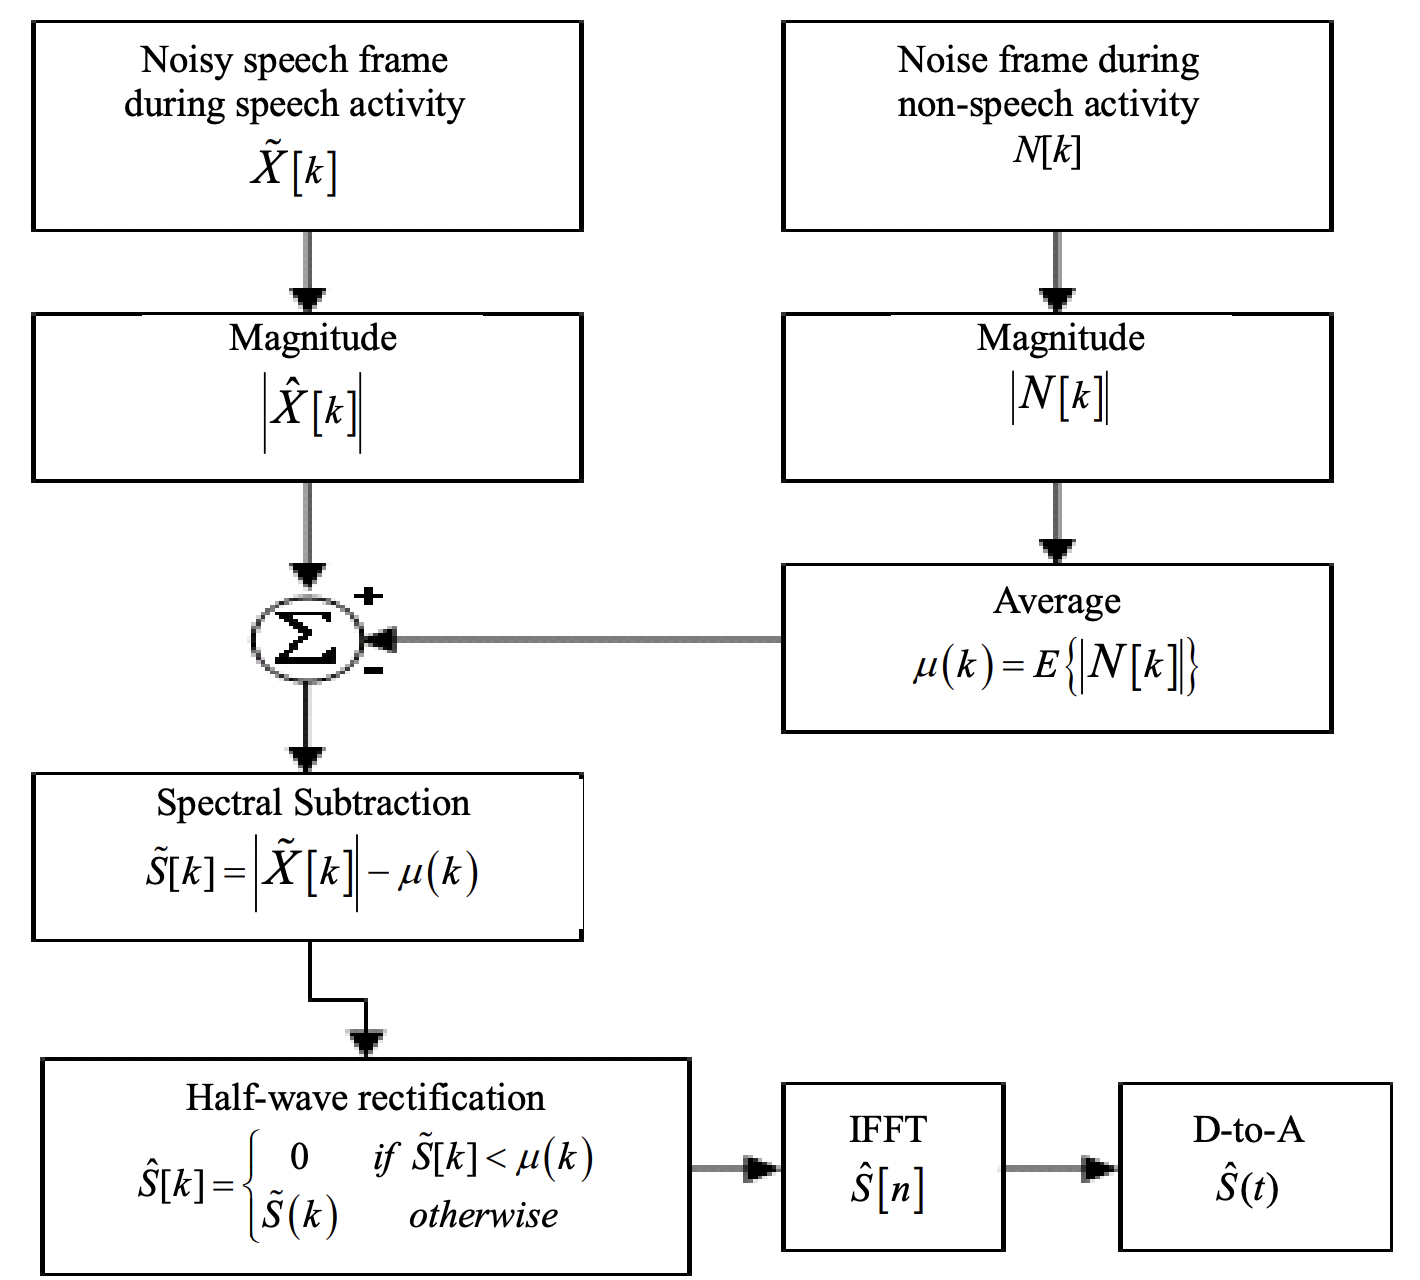
\includegraphics[scale=0.35]{spectralprocess.png}
	\caption{Spectral noise gating flowchart \cite{spectralflowchart}}
	\label{flowchart}
\end{figure}
The noise spectrum $N(\omega)$ and its statistical measures are obtained by asking users to record at least 3 seconds of silence 
before they sing into the app.
Note that half-wave rectification is necessary after noise removal process of subtracting the average magnitude of noise spectrum.
This is to target frequencies that have a higher average magnitude of noise spectrum $\textbf{E}[|N(\omega)|]$ compared to that of 
the noisy speech spectrum $|\hat{X(\omega)}|$. For those frequencies, we would replace the negative values with 0 with a half-wave 
rectification.

%-----------------------------------
%	SUBSECTION 3
%-----------------------------------

\subsection{Improvements}
A drawback with spectral reduction is that it does not handle extreme responses nicely. It does not reduce noises like
squeaks. Also, since a half-wave rectification is included in the implementation process, (Rao \& Sreelatha, 2014) has 
pointed out that residual noise will be created during the process of spectral reduction. Half-wave rectification introduces
nonlinearity in the $\hat{X(\omega)}$ spectrum and results in frequencies changing abruptly between frames.

As mentioned above, spectral reduction is built on the assumption that the noise is a stationary or slowly-varying. Yet in reality,
there may be sudden squeaky noise in the background which is not recorded in the noise profile. In this case, spectral reduction 
cannot remove the squeak. To improve the situation, we will introduce a low-pass filter to filter out high-frequency noise. The reason
for choosing LPF over a band-pass filter is that ambient noise is ususally low frequency and spectral reduction is effective 
in targeting the reduction of ambient noise. Thus as to avoid removing low-frequency desirable features, a low-pass filter will suffice.

To determine $f_c$ for the LPF, it would be plausible to refer to biological features of the users, i.e. their age and gender.
For males, the pitch level generally reduces from infancy to middle age, while a reversal of trend occurs after middle age. \cite{womenprange}
On the other hand, as pointed out by (Nishio & Niimi, 2008), "Females in their 30s and 40s showed obviously lower frequencies than those in their
20s. Across all age groups, including the 80s, fundamental frequencies tended to decrease markedly in association with aging”

\begin{table}
	\begin{minipage}{0.4\linewidth}
		\label{table:praat}
		\centering
		\begin{tabular}{lrr}		& Male   & Female  \\
			Pitch range (Hz)            & 60-180 & 160-300 \\
			Praat pitch range (Hz) 		& 50-300 & 100-600
		\end{tabular}
		\caption{Praat pitch range}
		\end{minipage}\hfill
	\begin{minipage}{0.55\linewidth}
		\centering
		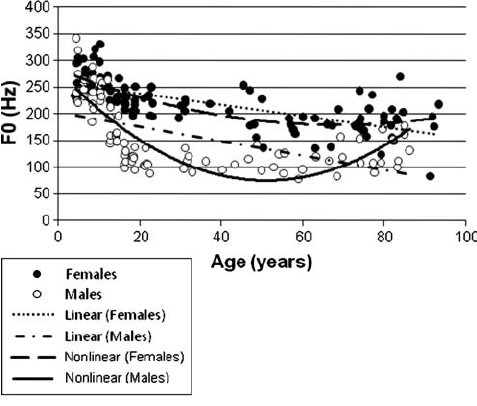
\includegraphics[scale=0.45]{f0vage.jpeg}
		\label{f0vage_chart}
		\captionof{figure}{Scatter plot of fundamental frequency by age \cite{f0age}}
	\end{minipage}
\end{table}

After referring to the measurements taken from 192 participants (Stathopoulos et al., 2011) and the pitch range
set by Praat (a software for speech analysis) \cite{praat}, a simple modelling of $f_c$ according to age and gender
is as below:
\[f_{c,male}(n) = 0.07n^2 - 7.5n + 280, for  4 <= n <= 93\]
\[f_{c,female}(n) = 0.02n^2 - 3n + 287, for  4 <= n <= 93\]
In deciding which filter to implement, there are 3 filters in consideration:
\begin{enumerate}[label=(\alph*)]
	\item Type 1 Chebyshev filter
	\[G_{n}(\omega) = |H_{n}(j\omega)| = {\frac{1}{\sqrt{1+\varepsilon^{2} T_{n}^{2}(\omega/\omega_{0})}}}\]
	where $\varepsilon$  is the ripple factor, $\omega _{0}$ is the cut-off frequency
	and $T_{n}$ is a Chebyshev polynomial of the $n$th order.
	\item Butterworth filter
	\[G_{n}(\omega) = |H_{n}(j\omega)| = {\frac{1}{sqrt{1+(\omega/\omega_{0})^{2n})}}}\]
	where $\omega _{0}$ is the cut-.off frequency and $n$ is the order of filter.
	\item Bessel filter
	\[G_{n}(\omega) = |H_{n}(j\omega)| ={\frac {\theta _{n}(0)}{\theta _{n}(j\omega/\omega _{0})}}\]
	where $\theta _{n}(j\omega)$ is a reverse Bessel polynomial and $\omega _{0}$ is the cut-off frequnecy
\end{enumerate}

Chebyshev filter has a steeper roll-off compared to Butterworth and Bessel filter, but it also brings passband and stopband ripples, 
unlike Butterworth and Bessel filter which have a flat passband and stopband as they roll-offs towards zero. Moreover, Butterworth 
and Bessel filters have a better step response. Meanwhile, Bessel filter performs the best in step response since the overshoot is
minimal. Also, an important characteristics Bessel filter has is that it introduces a linear-phase/ constant delay for $f<f_c$. This
feature allows us to preserve the waveshape since all frequencies are delayed by the same amount.
Thus, Bessel filter is preferred in this context.

\begin{figure}[h]
	\centering
	\begin{subfigure}{.32\textwidth}
	  	\centering
	  	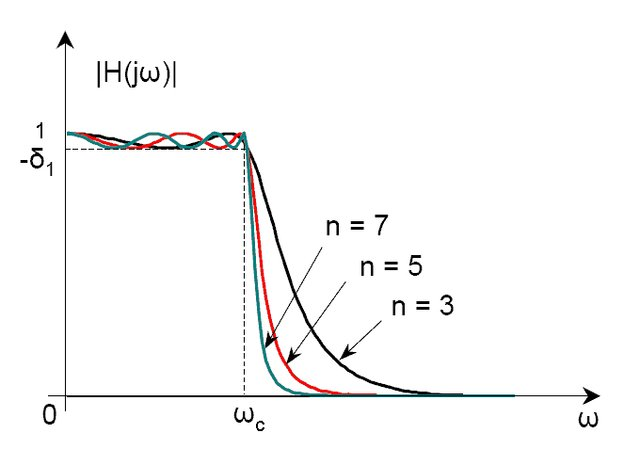
\includegraphics[width=1.1\linewidth]{chebyshev.jpeg}
	  	\caption{Type 1 Chebyshev filter frequency response}
	  	\label{fig:sub1}
	\end{subfigure}%
	\begin{subfigure}{.32\textwidth}
	  	\centering
	  	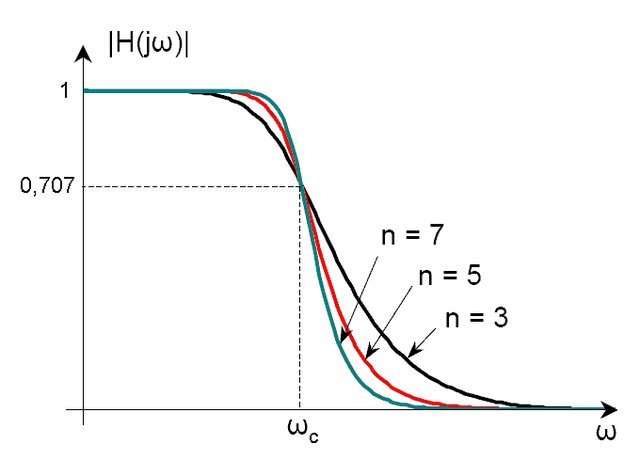
\includegraphics[width=1.1\linewidth]{butterworth.jpeg}
	  	\caption{Butterworth filter frequency response}
	  	\label{fig:sub2}
	\end{subfigure}
	\begin{subfigure}{.32\textwidth}
		\centering
		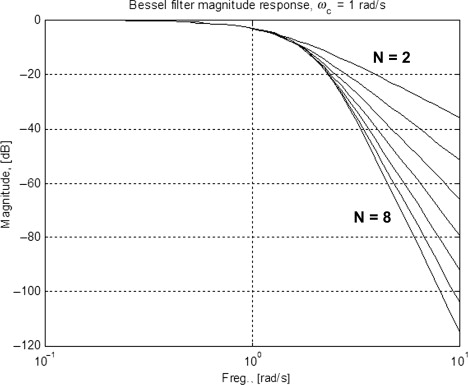
\includegraphics[width=1.1\linewidth]{bessel.jpg}
		\caption{Bessel filter frequency response \cite{bessel}}
		\label{fig:sub3}
	\end{subfigure}
\end{figure}

%----------------------------------------------------------------------------------------
%	SECTION 2
%----------------------------------------------------------------------------------------
\section{Pitch Detection Algorithm (PDA)}
After removing noise, we pass the processed signal to a PDA to estimate the fundamental frequency ($f0$) of
the signal.

%-----------------------------------
%	SUBSECTION 1
%-----------------------------------
\subsection{Possible Models}
There are 4 approaches to detect $f0$, which again can be classified into time domain and frequency domain.

\begin{enumerate}
	\item Zero crossings (time domain)
	This is the most intuitive method to detecting pitch although it suffers from low accuracy.
	Assuming the input is monophonic, the fundamental frequency is estimated as:
	\[f0 = \frac{P_{zcr}f_s}{2N}\]
	where $P_{Zcr}$ is the number of zero-crossing points, $f_s$ is the sampling rate,
	$N$ is the number of samples
	\begin{figure}{.6\textwidth}
		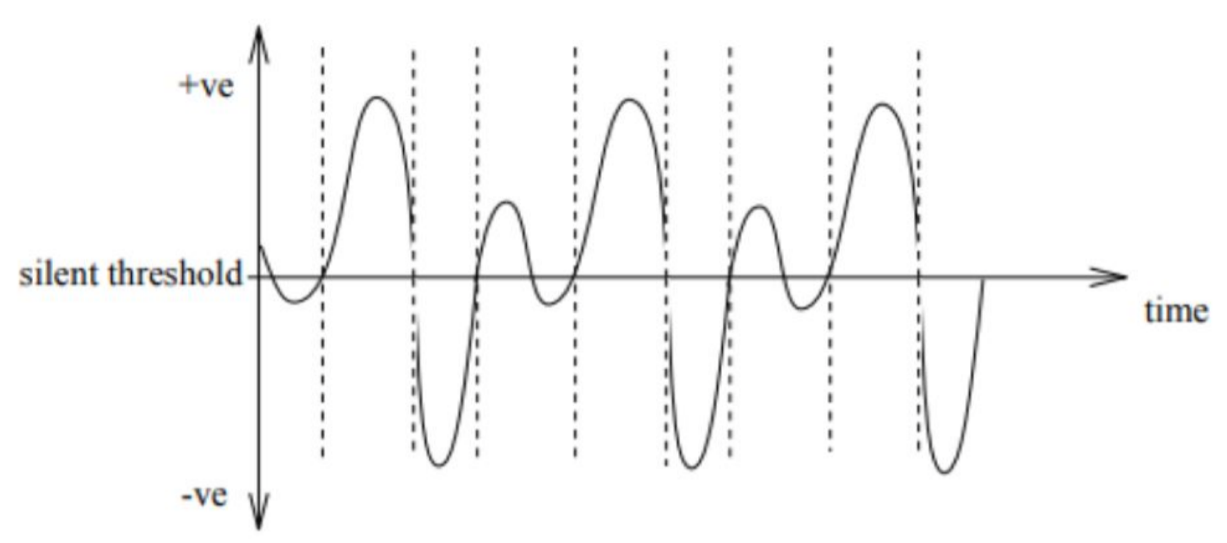
\includegraphics{zcr.png}
		\caption{An example signal with zero-crossings marked in dotted lines \cite{zcr}}
	\end{figure}
	
	\item YIN algorithm/ autocorrelation (time domain)
	As outlined by (de Cheveigné & Kawahara, 2002), YIN algorithm is based on a slightly altered autocorrelation method:
	\[r_t(\tau)=\sum_{j=t+1}^{t+W-\tau}x_j x_{j+\tau}\]
	where $r_t(\tau)$ is the autocorrelation function (ACF) of lag $\tau$ calculated at time index $t$, $W$ is the integration
	window size. Note that as $\tau$ increases, $W$ decreases and the envelope of the function decreases, as shown in figure 
	\textbf{INSERT}

	\begin{figure}
		\centering
		\begin{subfigure}{.3\textwidth}
		  \centering
		  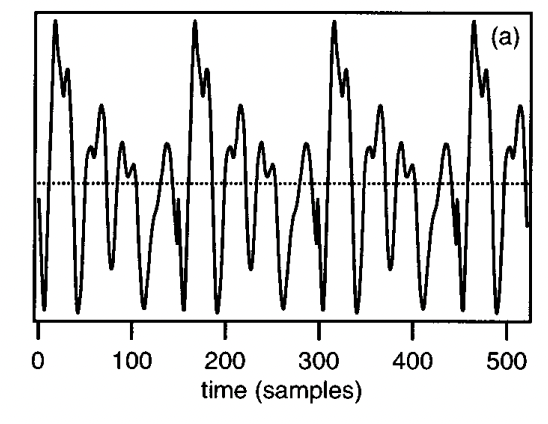
\includegraphics[width=1\linewidth]{signalwaveform.png}
		  \caption{Signal waveform}
		  \label{signal}
		\end{subfigure}%
		\begin{subfigure}{.3\textwidth}
			\centering
			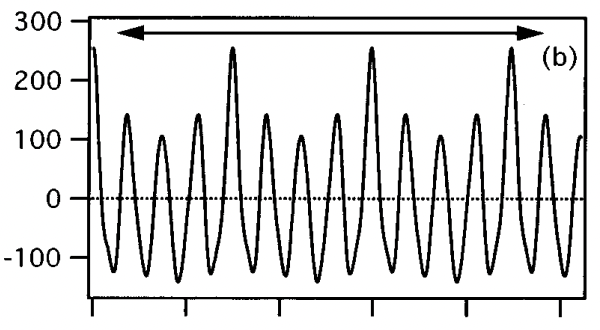
\includegraphics[width=1\linewidth]{acf.png}
			\caption{$r_t(\tau)$ calculated from figure \textbf{INSERT} using normal ACF}
			\label{acf}
		  \end{subfigure}%
		\begin{subfigure}{.3\textwidth}
		  \centering
		  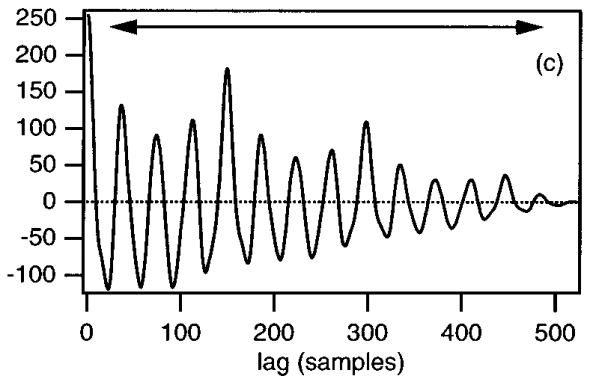
\includegraphics[width=1\linewidth]{taperedacf.png}
		  \caption{$r_t(\tau)$ calculated with the equation \textbf{INSERT}}
		  \label{taped}
		\end{subfigure}%
		\label{fig}
	\end{figure}
	
	We then select the highest peak by exhaustive search within an user-defined range of lags, the corresponding time lag will be
	the inverse of our estimated $f0$

	To improve the error rates and target periodicity, de Cheveigné & Kawahara introduced a cumulative mean normalized difference function (CMNDF)
	to replace ACF. 
	\[CMNDF(\tau) =  
	\begin{cases}
		1,              & \text{if } \tau \eq 0\\ 
    	\frac{DF(\tau)}{(1/\tau)\sum_{j=1}{\tau}DF(j)}, & \text{otherwise.} \\
	\end{cases}
	\]
	We then find $\tau$ that minimises $CMNDF(\tau)$ and the corresponding $f0$.

	\item Harmonic Product Spectrum (HPS) (frequency domain)
	As aforementioned, human voice is not of pure tone, a musical note sung will consist of a series of peaks in its frequency spectrum,
	which the peaks corresponds to $f0$ with other peaks indicating the harmonic components of integer multiples of $f0$. 
	Exploiting this fact, HPS algorithm creates multiple downsampled signal spectrums and compares them wiht the original spectrum as shown in figure 
	\textbf{INSERT}. The strongest harmonic peak will line up no matter how many times we compress the spectrum.
	
	\begin{figure}{.6\textwidth}
		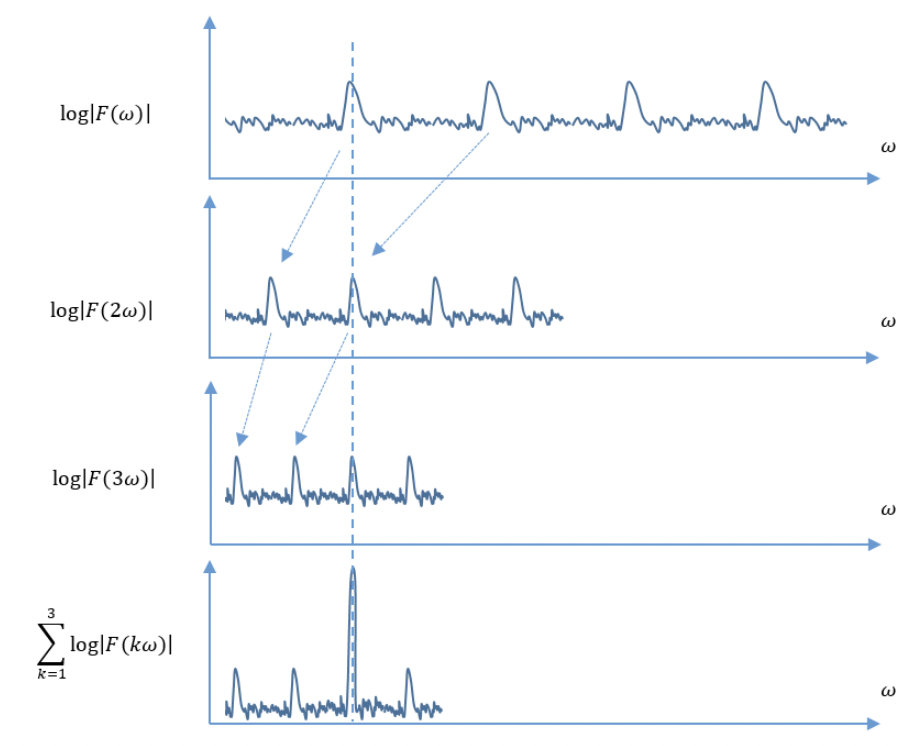
\includegraphics{HPS.png}
		\caption{Harmonically compressed log spectra \cite{HPS}}
	\end{figure}
	
	Firstly, we convolve the signal with a Hanning window to segment the input:
	\[w(n) = \frac{1+cos(2\pi n/N-1)}{2}, for 0<= n<= N-1\], where $N$ is the number of samples.
	We then convert it from time-domain to frequency-domain by computing the short-time Fourier Transform:
	\[STFT \{x[n]\}(k,\omega) = X(k,\omega )= \sum _{n=-\infty }^{\infty }x[n]w[n-k]e^{-j\omega n}\]
	Lastly we compute the product of spectrum at harmonics of a frequency and $f0$ is estimated by:
	\[f0 = argmax\prod_{k=1}^{n}|X(kf)|\] 

	\item CREPE (Convolutional Representation for Pitch Estimation)
	CREPE is a data-driven algorithm developed by (Kim et al., 2018) that operates directly on the time-domain.
	It consists of a deep convolutional neural network trained by synthesized audio from the RWC Music Database \cite{rwcdb}
	and MedleyDB \cite{medleydb}. %REFERENCE?

	The model is trained with 5-fold cross-validation and a 60/20/20 train, validation and test split.
	There are 6 convolutional layers and each layer is followed by a dropout layer with dropout probability of 0.25. 

	\begin{figure}{.6\textwidth}
		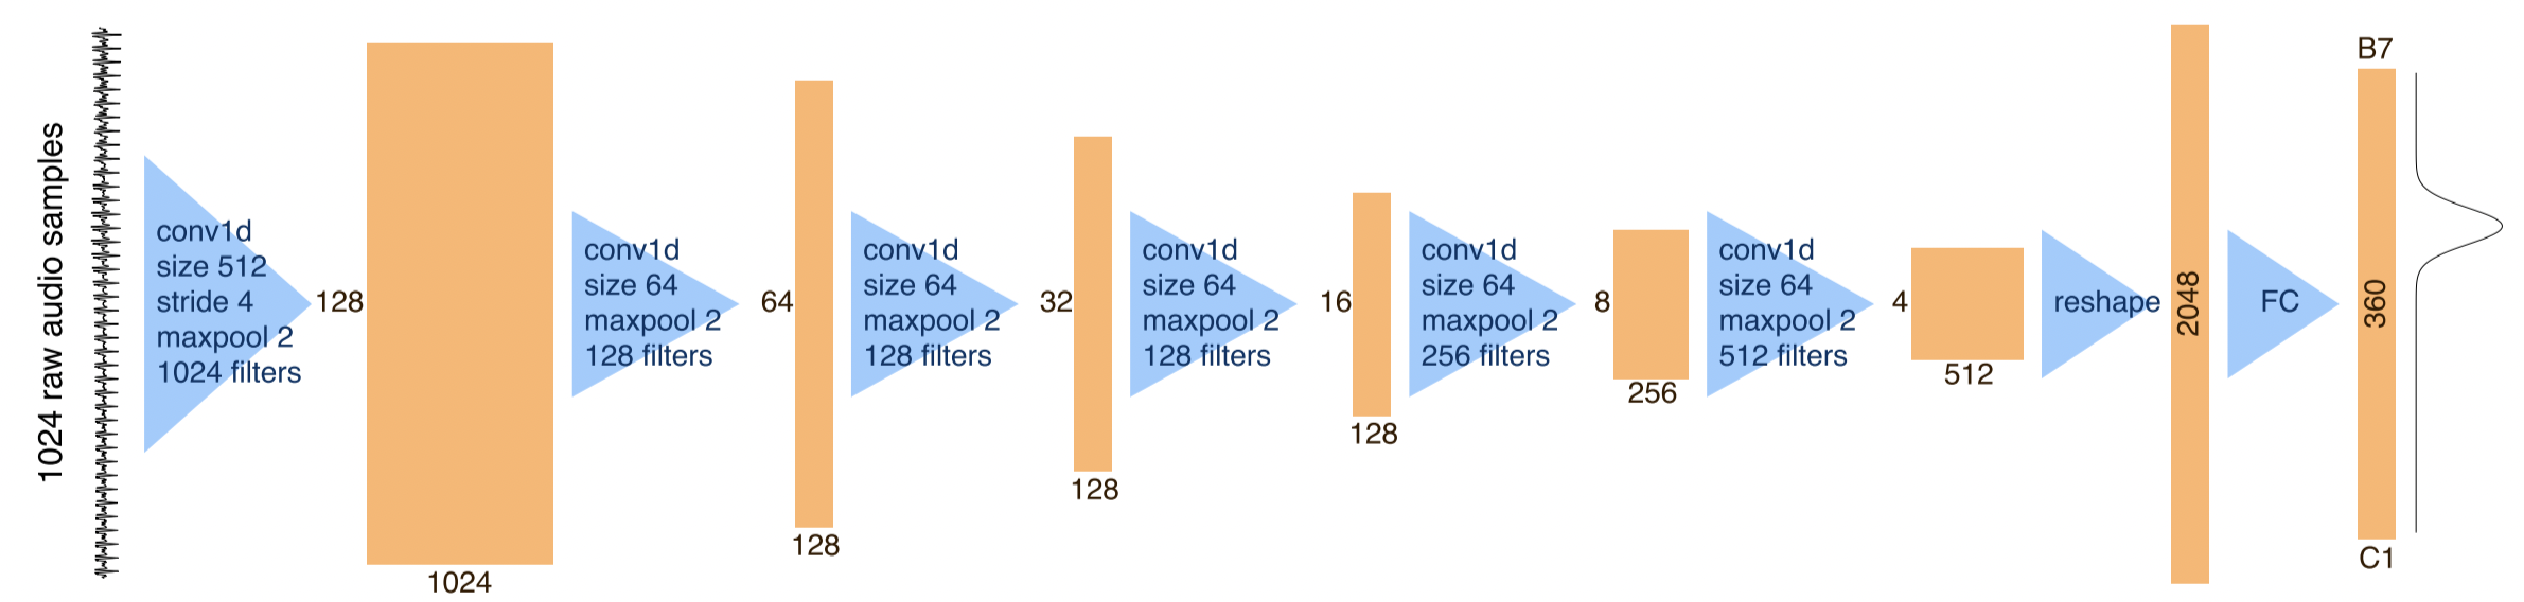
\includegraphics{CREPE.png}
		\caption{The architecture of the CREPE algorithm \cite{CREPE}}
	\end{figure}


\end{enumerate}



%-----------------------------------
%	SUBSECTION 2
%-----------------------------------
\subsection{Comparison between models and implementation}
The zero crossings method will not be considered since it heavily relies on the assumption that the input audio is of pure tone. Yet,


"the human voice is not a pure tone (as produced by a tuning fork); rather, it is composed of a fundamental tone (or frequency of vibration) and a series of higher frequencies called upper harmonics," \cite{humanmono}

acf- range of lags have to be considered ( if too small, choose zero lag peak. if too high, erroneously choose a higher order peak that is far apart)

HPS - Pros: HPS is simple to implement, does well under a wide range of conditions, and runs in real-time.

Cons: low frequency resolution must be enhanced by zero-padding, so that the spectrum can be interpolated to the nearest semitone. This means that high frequencies are also being unecessarily interpolated.

only works well for signals that have a full set of harmonics with sufficient magnitudes.
or can add a suitably large non-zero floor to all harmonic magnitudes being multiplied together.

Another severe shortfall of the HPS method is that it its resolution is only as good as the length of the FFT used to calculate the spectrum. If we perform a short and fast FFT, we are limited in the number of discrete frequencies we can consider. In order to gain a higher resolution in our output (and therefore see less graininess in our pitch output), we need to take a longer FFT which requires more time.



%-----------------------------------
%	SUBSECTION 3
%-----------------------------------

\subsection{Improvements}
(find an algorithm to take in users’ singing frequency to improve accuracy of the model ( perhaps adjust the likelihood of the crepe model?) ( look into automl)

%----------------------------------------------------------------------------------------
%	SECTION 3
%----------------------------------------------------------------------------------------
\section{Key Detection Algorithm (KDA)}

%-----------------------------------
%	SUBSECTION 1
%-----------------------------------
\subsection{Possible Models}

%-----------------------------------
%	SUBSECTION 2
%-----------------------------------

\subsection{Implementation}
